\documentclass[conference]{IEEEtran}

\usepackage{graphicx}
\usepackage{booktabs}
\usepackage{array}
\usepackage{url}
\usepackage{float}

\title{Tox21 Molecular Toxicity Prediction Using an MLOps Deployment Pipeline}

\author{
\IEEEauthorblockN{Author Name: TODO}
\IEEEauthorblockA{
Department / Program: TODO\\
Institution: TODO\\
Email: TODO
}
}

\begin{document}
\maketitle

\begin{abstract}
This report presents an end-to-end MLOps pipeline for molecular toxicity prediction using the Tox21 dataset. The project converts molecular SMILES strings into 1024-bit Morgan fingerprints with RDKit, trains and compares Logistic Regression, Random Forest, and Extra Trees classifiers, tracks experiments with MLflow, serves the selected model through FastAPI, and exposes operational metrics through Prometheus and Grafana. The selected model predicts the SR-ARE toxicity endpoint and is packaged with Docker, validated through GitHub Actions CI, and published through a GitHub Container Registry image workflow.
\end{abstract}

\begin{IEEEkeywords}
MLOps, Tox21, molecular toxicity prediction, FastAPI, Docker, MLflow, Prometheus, Grafana, GitHub Actions
\end{IEEEkeywords}

\section{Introduction}
Molecular toxicity prediction is an important machine learning use case in computational drug discovery and chemical safety screening. This project focuses on building a reproducible MLOps workflow around a Tox21 binary classification task rather than only training a standalone model.

The implemented system predicts the \texttt{SR-ARE} endpoint from molecular SMILES strings. The repository includes the dataset, training pipeline, selected model artifact, FastAPI inference service, Docker configuration, Prometheus metrics, Grafana dashboard provisioning, CI validation, and CD image publishing workflow.

\section{System Architecture}
Fig.~\ref{fig:architecture} shows the high-level architecture of the implemented pipeline. The workflow is divided into data and model development, deployment and orchestration, and client and observability components.

\begin{figure*}[t]
    \centering
    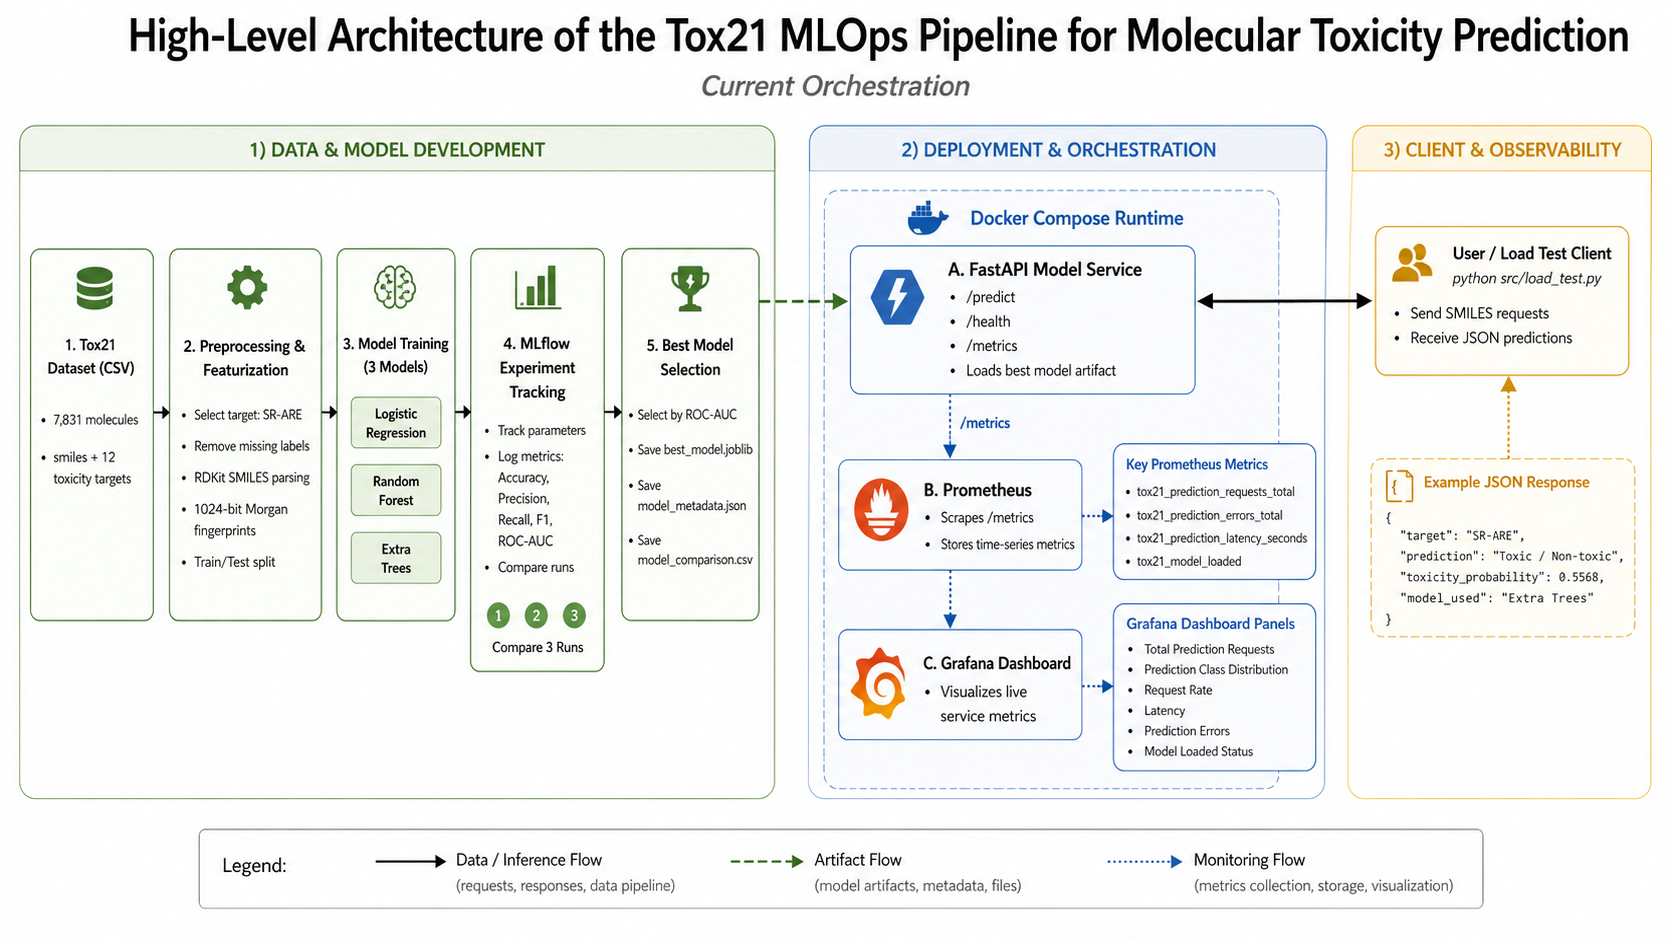
\includegraphics[width=0.98\textwidth]{../High_Level_Design.png}
    \caption{High-level architecture of the Tox21 MLOps pipeline for molecular toxicity prediction.}
    \label{fig:architecture}
\end{figure*}

The training stage reads \texttt{data/tox21.csv}, preprocesses molecules, generates Morgan fingerprints, trains three models, logs runs to MLflow, and saves the best model artifact. The serving stage uses FastAPI inside a Docker-based runtime. Prometheus scrapes the API's \texttt{/metrics} endpoint, and Grafana visualizes service health, prediction traffic, request quality, and latency.

\section{Dataset and Feature Engineering}
The project uses the Tox21 dataset stored as a CSV file. The training script selects the \texttt{SR-ARE} target column and removes records with missing target labels. SMILES strings are parsed using RDKit. Molecules that cannot be parsed are skipped during training.

Each valid molecule is represented as a 1024-bit Morgan fingerprint with radius 2. The same fingerprint generation logic is used by the FastAPI service at inference time, ensuring that the training and serving paths use the same feature representation.

\begin{table}[H]
\centering
\caption{Dataset and Feature Configuration}
\label{tab:data}
\begin{tabular}{ll}
\toprule
\textbf{Item} & \textbf{Value} \\
\midrule
Dataset & Tox21 \\
Input format & CSV \\
Target column & \texttt{SR-ARE} \\
Molecular input & SMILES string \\
Feature type & Morgan fingerprints \\
Fingerprint size & 1024 bits \\
Fingerprint radius & 2 \\
\bottomrule
\end{tabular}
\end{table}

\section{Model Training and Selection}
The training pipeline compares three classical machine learning models: Logistic Regression, Random Forest, and Extra Trees. A stratified train-test split is used, and model performance is evaluated using accuracy, precision, recall, F1 score, and ROC-AUC.

The selected model is Extra Trees, chosen using ROC-AUC as the selection metric. The selected model is saved as \texttt{models/tox21\_best\_model.joblib}, and metadata is stored in \texttt{models/model\_metadata.json}.

\begin{table}[H]
\centering
\caption{Model Evaluation Results}
\label{tab:metrics}
\begin{tabular}{lccccc}
\toprule
\textbf{Model} & \textbf{Acc.} & \textbf{Prec.} & \textbf{Rec.} & \textbf{F1} & \textbf{AUC} \\
\midrule
Logistic Regression & 0.7494 & 0.3443 & 0.6117 & 0.4406 & 0.7443 \\
Random Forest & 0.7923 & 0.3846 & 0.4787 & 0.4265 & 0.7592 \\
Extra Trees & 0.7700 & 0.3571 & 0.5319 & 0.4274 & 0.7648 \\
\bottomrule
\end{tabular}
\end{table}

\begin{figure}[H]
    \centering
    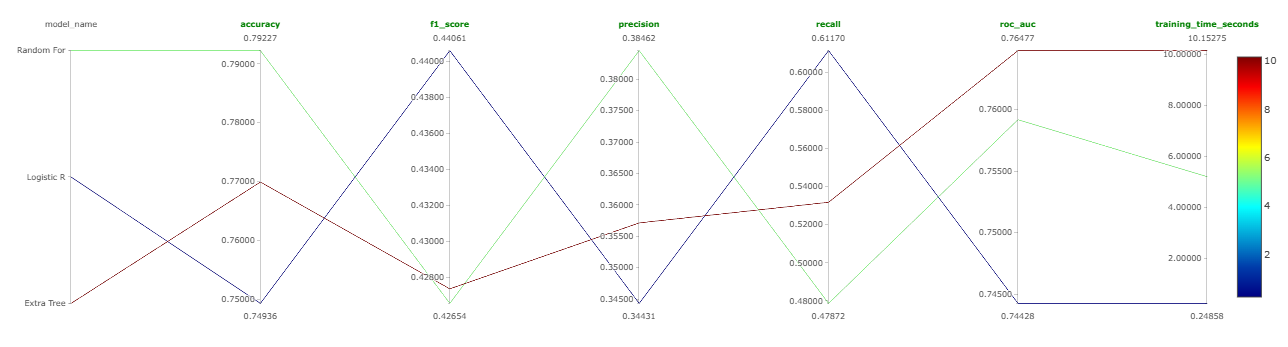
\includegraphics[width=0.48\textwidth]{../Images_ForGPT/MLFLOW.PNG}
    \caption{MLflow experiment tracking screenshot captured from the project artifacts.}
    \label{fig:mlflow-runs}
\end{figure}

\section{API Serving Layer}
The inference service is implemented with FastAPI in \texttt{app/main.py}. The API loads the selected model artifact at startup and exposes the endpoints shown in Table~\ref{tab:api}.

\begin{table}[H]
\centering
\caption{FastAPI Endpoints}
\label{tab:api}
\begin{tabular}{ll}
\toprule
\textbf{Endpoint} & \textbf{Purpose} \\
\midrule
\texttt{GET /} & Service root message \\
\texttt{GET /health} & Model and service health metadata \\
\texttt{GET /version} & App, model, and runtime version metadata \\
\texttt{POST /predict} & Toxicity prediction for a SMILES input \\
\texttt{GET /metrics} & Prometheus-compatible service metrics \\
\bottomrule
\end{tabular}
\end{table}

The \texttt{/predict} endpoint accepts a JSON payload containing a SMILES string. Valid inputs return the target, predicted toxicity label, probability estimate, selected model name, and model version. Invalid SMILES strings are rejected with an HTTP 400 response.

\section{Observability}
The API exposes Prometheus metrics for prediction attempts, prediction outcomes, prediction errors, response status codes, prediction latency, and model load status. These metrics support operational visibility into request volume, invalid inputs, server errors, and latency behavior.

Grafana provisioning is included in the repository. The dashboard is grouped around service health, traffic quality, and latency so that panels reflect the available metrics rather than arbitrary visualizations.

Fig.~\ref{fig:grafana-dashboard} shows the current dashboard view included with the project artifacts.

\begin{figure}[H]
    \centering
    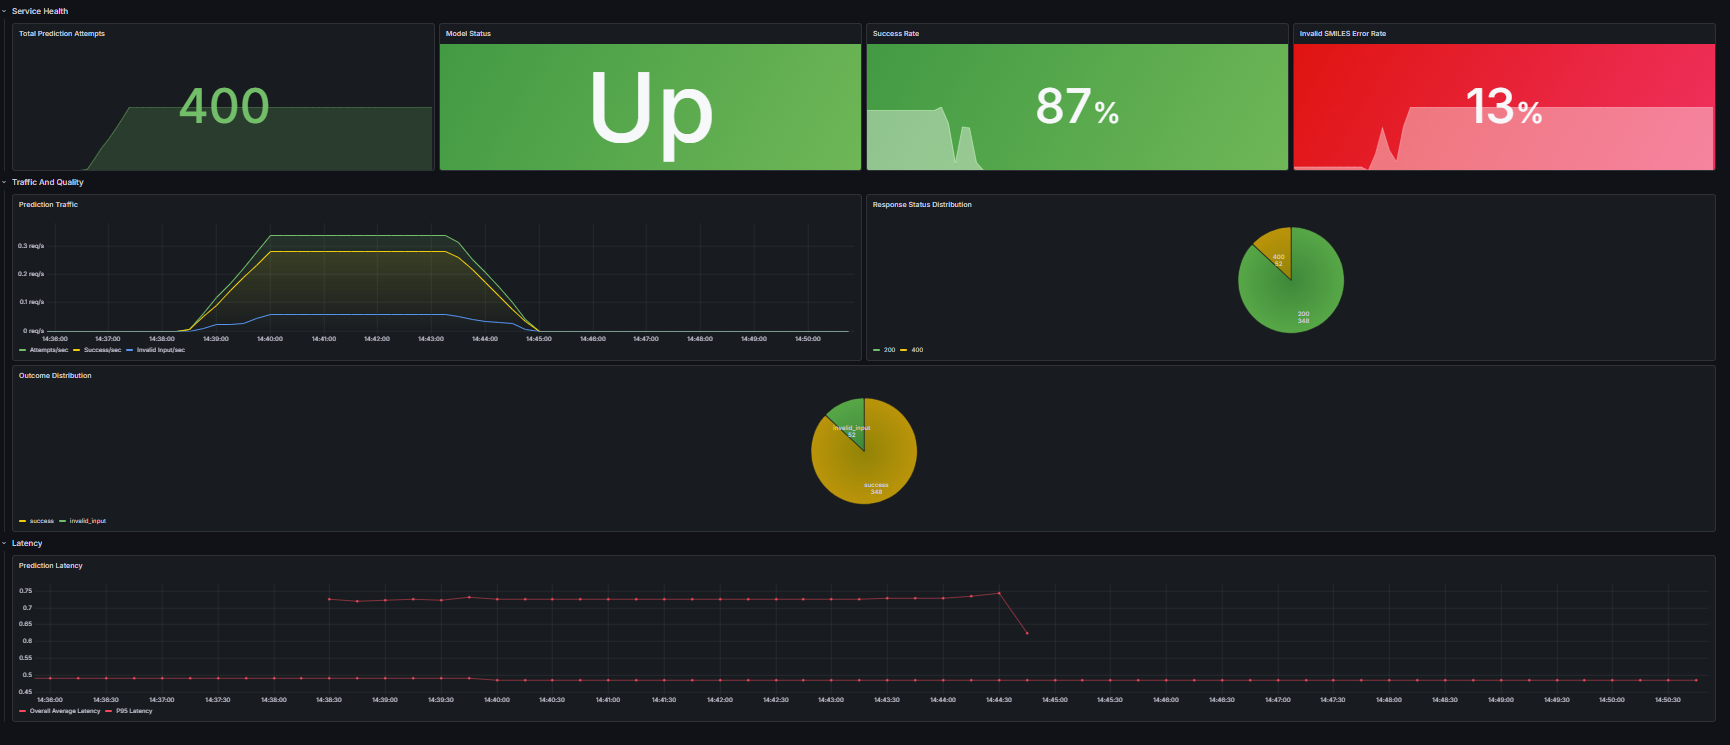
\includegraphics[width=0.48\textwidth]{../Images_ForGPT/Grafana.PNG}
    \caption{Grafana dashboard screenshot captured from the project artifacts.}
    \label{fig:grafana-dashboard}
\end{figure}

\begin{table*}[t]
\centering
\caption{Prometheus Metrics Exposed by the API}
\label{tab:prometheus}
\footnotesize
\begin{tabular}{p{0.40\textwidth}p{0.52\textwidth}}
\toprule
\textbf{Metric} & \textbf{Purpose} \\
\midrule
\texttt{tox21\_prediction\_requests\_total} & Successful predictions by label \\
\texttt{tox21\_prediction\_attempts\_total} & Total prediction attempts \\
\texttt{tox21\_prediction\_outcomes\_total} & Outcomes such as success and invalid input \\
\texttt{tox21\_prediction\_errors\_total} & Prediction errors by type \\
\texttt{tox21\_prediction\_status\_codes\_total} & Responses by HTTP status code \\
\texttt{tox21\_prediction\_latency\_seconds} & Prediction latency histogram \\
\texttt{tox21\_model\_loaded} & Model load status gauge \\
\bottomrule
\end{tabular}
\end{table*}

\section{CI/CD and Reproducibility}
GitHub Actions is used for CI and CD. The CI workflow runs on pushes and pull requests targeting \texttt{main}. It installs pinned dependencies, verifies required files, compiles Python files, runs tests, checks model artifact compatibility with the runtime scikit-learn version, and builds the Docker image on pushes.

The CD workflow publishes the API Docker image to GitHub Container Registry. It supports branch, tag, semantic version, latest, and SHA-based image tags. The workflow also includes an optional deploy webhook step controlled by the \texttt{DEPLOY\_WEBHOOK\_URL} secret.

Runtime reproducibility is improved by pinning dependencies and recording training library versions in \texttt{models/model\_metadata.json}. The current model metadata records Python 3.11.9 and scikit-learn 1.8.0 for the training environment, and the API reports both training and runtime scikit-learn versions.

\section{Limitations}
This project is intended as an MLOps demonstration and should not be treated as a validated toxicology decision system. The model is specific to the \texttt{SR-ARE} endpoint, uses fixed molecular fingerprints rather than learned molecular representations, and reports moderate evaluation metrics. Any real-world scientific, clinical, regulatory, or safety-critical use would require stronger validation, calibration analysis, monitoring, data governance, and domain expert review.

\section{Conclusion}
The project demonstrates a complete MLOps workflow for molecular toxicity prediction: data preprocessing, feature generation, model comparison, experiment tracking, artifact management, API serving, containerization, observability, CI validation, and image publishing. The implemented pipeline provides a reproducible foundation for demonstrating how machine learning models can be operationalized beyond notebook-based experimentation.

\section*{Missing Information To Complete Final Submission}
The following academic metadata was not available in the repository and should be filled before final submission:

\begin{itemize}
    \item Author name
    \item Institution or department
    \item Course or module name
    \item Instructor or supervisor name
    \item Submission date
    \item Required citation style or references, if mandated by the course
\end{itemize}

\end{document}
